\documentclass[11pt]{report}
\usepackage{textcomp}
\usepackage{amsmath}

\usepackage{titlesec}
\titlespacing*{\section}
{0pt}{\baselineskip}{0em}
\titlespacing*{\subsection}
{0pt}{\baselineskip}{0em}

\usepackage{geometry}
\geometry{left=1in, right=1in, top=1in, textheight=9in}

\usepackage{enumitem}
\newlist{steps}{enumerate}{1}
\setlist[steps, 1]{wide=0pt, leftmargin=\parindent, label=Step \arabic*:}

\usepackage{fancyhdr}
\fancypagestyle{plain}{%
    \fancyhf{} % clear all header and footer fields
    \fancyfoot[C]{\sffamily\fontsize{.75em}{.75em}\selectfont\thepage} % except the center
    \renewcommand{\headrulewidth}{0pt}
    \renewcommand{\footrulewidth}{0pt}
}
\pagestyle{plain}

\usepackage{graphicx}
\graphicspath{ {./media/} }

\usepackage{setspace}
\doublespacing

\usepackage{minted}
\usepackage{xcolor}
\definecolor{inlinebg}{rgb}{0.95, 0.95, 0.95}
\newmintinline[vhdl]{vhdl}{fontsize=\small, bgcolor=inlinebg}

% make fancy title page
\makeatletter
\newcommand{\@labsection}{000}
\newcommand{\labsection}[1]{
    \renewcommand{\@labsection}{#1}
}

\newcommand{\@labnumber}{0}
\newcommand{\labnumber}[1]{
    \renewcommand{\@labnumber}{#1}
}

\newcommand{\@shortsubmitted}{1/1/70}
\newcommand{\shortsubmitted}[1]{
    \renewcommand{\@shortsubmitted}{#1}
}

\lfoot{\footnotesize \textit{University of Arkansas \\ EECS Department}}
\rfoot{\footnotesize \textsl{\@shortsubmitted}}

\renewcommand{\maketitle}{
    \newgeometry{left=1in, right=1in, top=1.75in, textheight=8.25in}
    \singlespacing
    \begin{center}
        {\huge \bf CSCE 22104} \\
        \vspace{2.5em}
        {\Large \bf Lab Report} \\
        \vspace{2em}
        \noindent\rule{20em}{0.4pt} \\
        \vspace{1em}
        {\Large \@author} \\
        \vspace{.75em}
        {\normalsize ID: 011019116} \\
        \vspace{.75em}
        {\normalsize Lab Section \@labsection} \\
        \vspace{.75em}
        {\normalsize Lab \@labnumber}
    \end{center}
    \newpage
    \restoregeometry
}

\makeatother

\newcommand*{\xor}{\oplus}

% TEXTWIDTH = 100
\begin{document}
\author{Brent Marcus Orlina}

\labsection{001}
\labnumber{2}

\shortsubmitted{2/5/25}

\maketitle

\section*{Introduction}
This lab's goal was to create a full-adder component and a 4-bit ripple carry adder component. The
full-adder should be able to add two bits along with an extra bit, \verb|cin| in the case that
there is an incoming carry bit. The output should be the sum of the input bits and another bit,
\verb|cin| to signal that there is a carry onto the next digit in the sum.

The 4-bit ripple carry adder should be able to add two 4-bit numbers. The output should be the sum
of the two 4-bit numbers and another bit, \verb|cout|, to signal that there was a carry in the sum
of the last digit. The ripple carry adder also has an extra input bit, \verb|cin| in the case that
there is an incoming carry bit from some other adder.

\section*{Approach}
In the addition of two bits $A$ and $B$, all the possibilities of $A$ and $B$ can feasibly be
considered. Its truth table looks like
\begin{center}
\begin{tabular}{ |c|c|c| } 
 \hline
 $A$ & $B$ & $A + B$ \\ 
 \hline
 0 & 0 & 0 \\ 
 0 & 1 & 1 \\ 
 1 & 0 & 1 \\ 
 1 & 1 & 0 \\ 
 \hline
\end{tabular}
\end{center}

The truth table is identical to the XOR operation in boolean algebra, therefore the XOR operation
can model bit-addition. The XOR operation is also associative and thus is able to add three bits
together without worrying about order. In the end, the sum of the three input bits of the full-adder
can be expressed as
\begin{equation}
    S = A \xor B \xor C_{in} \label{eq:sum}
\end{equation}
where $A$ and $B$ are the two input bits and $cin$ is the extra incoming carry bit.

In addition, the concept of a ``carry'' is to signal that the sum of a digit is too large to fit in
a single digit and thus must be ``carried'' and added onto the next digit. In bit addition, the sum
of two $1$'s is too large for a single digit to represent and thus must be carried onto the next
digit. Therefore, checking if there are at least two $1$'s being added  is enough to know if there
should be a carry onto the next digit. In boolean algebra, it can be expressed as
\begin{equation}
    C_{out} = (A \land B) \lor (A \land C_{in}) \lor (B \land C_{in}) \label{eq:cout}
\end{equation}

The full-adder was built by following the two previous equations. A \verb|GateXOR|, \verb|GateAND|,
and \verb|GateOR| were made so that the full-adder was built structurally. The \verb|GateXOR| and
\verb|GateOR| was made such that it had three inputs and did the respective binary operation of each
input in order. E.g. the \verb|GateOR| had the output of \vhdl{A xor B xor C} where \verb|A|,
\verb|B|, and \verb|C| are the three inputs.

The 4-bit ripple carry adder was built structurally by using four full-adders. Each bit of the input
bits is connected to a full-adder. E.g. the first bit of inputs \verb|A| and \verb|B| are connected
to the first full-adder, the second bits are connected to the second full-adder, and so on. The
first full-adder's \verb|cout| is connected to the second full-adder's \verb|cin|. The second
full-adder's \verb|cout| is connected to the third full-adder's \verb|cout|, and so on for the third
and fourth full-adder. The ripple carry adder's input bit \verb|cin| is connected to the first
full-adder's \verb|cin| and the last full-adder's \verb|cout| is connected to the ripple carry
adder's output bit \verb|cout|.

\section*{Experimentation}
The components' behaviors were tested using hand-crafted testbenches. The testbench for the
full-adder component tested all possible combinations of the input bits. The full-adder worked as
expected and follows the equations \eqref{eq:sum} and \eqref{eq:cout}. 

The testbench for the 4-bit ripple carry adder did not test for all possibilities of the inputs.
However, it is sufficient enough as it tests addition with \verb|cin| active and inactive and
overflowing addition with \verb|cin| active and inactive. The 4-bit ripple carry adder worked as
expected, displaying the correct sum of the input bits. Inputs in which the sum does not fit in four
bits correctly activates the output bit \verb|cout| and the resulting sum loops back around.

\newpage

\section*{Results \& Discussion}
\begin{figure}[h!]
    \centering
    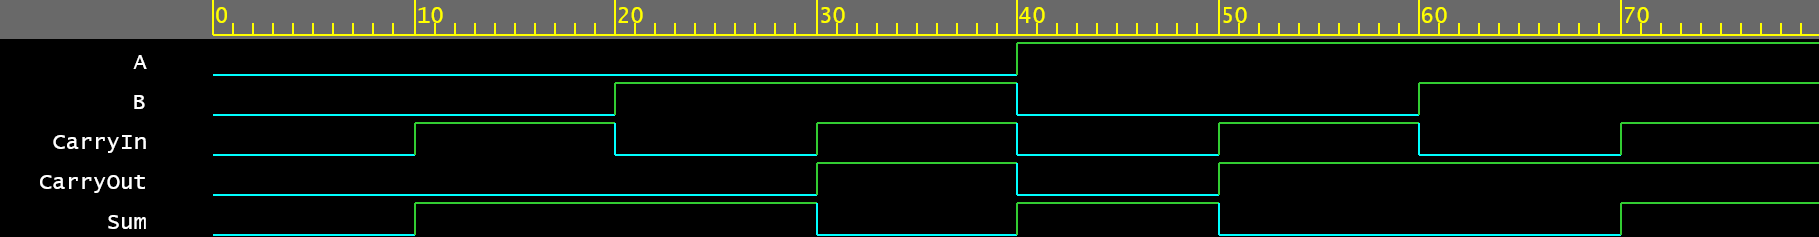
\includegraphics[width=0.95\textwidth]{FullAdder-waveform}
    \caption{
        The waveform for the full-adder component implementation.
    }
    \label{fig:FullAdder-waveform}
\end{figure}

The full-adder component works as expected. In figure \ref{fig:FullAdder-waveform}, it shows that
when only one of the input bits are active, the \verb|Sum| is active and \verb|CarrOut| is inactive.
When only two of the input bits are active, \verb|CarryOut| is active and \verb|Sum| is inactive.
When all three input bits are active, both \verb|Sum| and \verb|CarryOut| are active. This follows
both equations \eqref{eq:sum} and \eqref{eq:cout}. The testbench for this component is sufficient
since it has tested all possible combinations of the input bits.

\begin{figure}[h!]
    \centering
    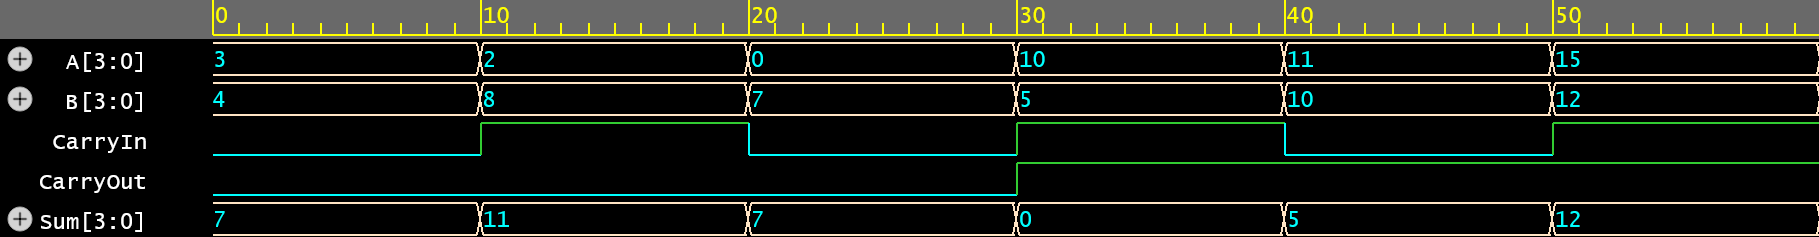
\includegraphics[width=0.95\textwidth]{RCA4-waveform}
    \caption{
        The waveform for the 4-bit ripple carry adder implementation.
    }
    \label{fig:RCA4-waveform}
\end{figure}

The 4-bit ripple carry adder also works as expected. In figure \ref{fig:RCA4-waveform}, it shows
the addition of \verb|A| and \verb|B| with the result in \verb|Sum|. From 0ns to 10ns, it shows $3 +
4$ correctly showing the sum of $7$ with the \verb|CarryOut| inactive. From 10ns to 20ns, it shows
the $2 + 8$ with the input bit \verb|CarryIn| active. It correctly shows the sum of $11$, with
\verb|CarryOut| inactive, and not $10$ since the \verb|CarryIn| input is active, thus adding an
extra $1$. The cases from 30ns to 60ns shows cases of overflow with each one correctly showing the
results with \verb|CarryOut| active. These cases overflow because there aren't enough bits to
represent the sum of the two numbers. For example, the 5-bit representation of the case from 40ns to
50ns would be
\[
    \texttt{01011} + \texttt{01010} = \texttt{10101}
\]
correctly, resulting in the binary form of $21$. However, the adder only has four bits, so the
leftmost bit is ``thrown away'', leaving only \verb|0101|, or $5$ in decimal form. This has the same
effect of doing modular arithmetic in mod $2^4$, or mod $16$.
\begin{align*}
    11 + 10 &\equiv 21 \pmod{16} \\
            &\equiv 5  \pmod{16}
\end{align*}

Although the testbench for the 4-bit ripple carry adder did not test for all possible combinations
of the inputs, it is sufficient enough since it tests for addition with \verb|CarryIn| both active
and inactive and overflowing addition with \verb|CarryIn| both active and inactive.

\section*{Conclusions}
Both the full-adder component and the 4-bit ripple carry adder displayed the correct behavior during
testing. The knowledge learned from this lab was learning how a full-adder and 4-bit ripple carry
adder works and how to construct them structurally, using the full-adder component to make the 4-bit
ripple carry adder. The skills practiced in this lab was learning how to build components
structurally and create sufficient testbenches.

% \newpage
% 
% \section*{References}
% \noindent
% [1]    Computer Organization 22104, EECS, University of Arkansas, “Lab 1,”  Sep. 17, 2024.
% 
% \noindent
% [2]    Computer Organization 22104, EECS, University of Arkansas, “Lab 2,”  Sep. 24, 2024.
% 
% \newpage
% 
% \section*{Appendix}
% \begin{figure}[h!]
%     \centering
%     \includegraphics[width=0.9\textwidth]{foo}
%     \caption{
%         Lorem ipsum dolor sit amet, qui minim labore adipisicing minim sint cillum sint consectetur
%         cupidatat.
%     }
%     \label{fig:foo}
% \end{figure}
% 
% \newpage
% 
% \begin{figure}[h!]
%     \centering
%     \includegraphics[height=0.4\textheight]{bar}
%     \caption{Lorem ipsum something something shorter sentence}
%     \label{fig:bar}
% \end{figure}
\end{document}
